\documentclass[preview,border=5pt]{standalone}
\usepackage{teaching}
\begin{document}

\centering

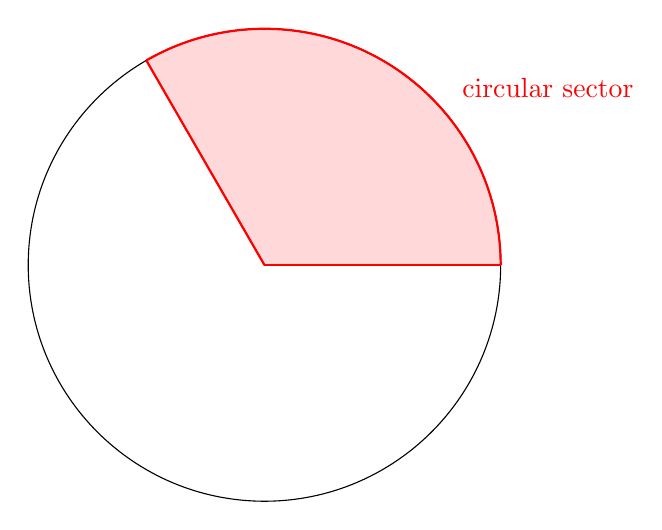
\begin{tikzpicture}[yscale=1,xscale=1,scale=1.5,inner sep=0.1mm, label distance=1.5mm]

%\draw[black!30!white, ->] (-3,0) -- (3,0);
%\draw[black!30!white, ->] (0,-3) -- (0,3);
%\node(t) at (3.15,0) [color=black!50!white] {$x$};
%\node(t) at (0,3.15) [color=black!50!white] {$y$};
\draw[fill=red!15!white] (0,0) -- (2,0) arc (0:120:2cm)  -- (0,0);
\draw (0,0) circle (2);
%\draw[color=red!70!white] (0.5,0) arc (0:57.2958:0.5cm);
\draw[red,thick] (0,0) -- (2,0);
\draw[red,thick] (0,0) -- (-1,1.73205080757);
\draw[red,thick] (2,0) arc (0:120:2cm);
%\node(l) at (2.2,1.1) [color=red] {$r$};
%\node(r) at (1,-0.2) [color=red] {$r$};
%\node(j) at (0.5,1.2) [color=red] {$r$};
\node(j) at (2.4,1.5) [color=red] {circular sector};

\end{tikzpicture}

\end{document}